\section{Convention Centre}\label{sec:Convention Centre} % (fold)

Here I will explicitly list out the conventions used in this note.
\begin{itemize}
  \item \textbf{Infinitesimal Conformal Transformation} We use the
    convention in the yellow book:
    \begin{align}
      z &\to z' = z + \epsilon(z) \\
      \bar{z} &\to \bar{z}' = \bar{z} + \bar{\epsilon}(\bar{z})
    \end{align}
    which gives:
    \begin{align}
      \delta_{\epsilon,\bar{\epsilon}} \phi(z,\bar{z}) = - \left[
        \epsilon(z) \partial_z + h \partial_z \epsilon(z) +
        \bar{\epsilon}(\bar{z}) \partial_{\bar{z}} + \bar{h}
      \partial_{\bar{z}} \bar{\epsilon}(\bar{z}) \right] \phi(z,\bar{z})
    \end{align}
    For the primary fields.
  \item \textbf{Holomorphic coordinate} This is the standard definition

  \item \textbf{Holomorphic E-M tensor} there are two commonly used
    convention, we always take the yellow book convention:
    \begin{align}
      \quad T(z) = -2 \pi T_{zz} \quad \bar{T}(\bar{z}) = -2 \pi
      T_{\bar{z}\bar{z}}
    \end{align}
    Different convention never changes the definition of $ T(z) $ to
    ensure the same form of OPEs and Ward Identities.
  \item \textbf{Conformal Generators} are defined as the following
    comutation relation and the consistent exp map:
    \begin{align}
      -[Q,\phi] = \delta_{\epsilon,\bar{\epsilon}} \phi
    \end{align}
  \item \textbf{Relation between E-M tensor and Hamiltonian}

    Hamiltonian can be written in the following convention:
    \begin{align}
      H = \int \displaystyle\frac{1}{2 \pi} T_{tt} dx
    \end{align}
    \YL{[I'll prove its consistency later.]}
\end{itemize}

% section Convention Centre (end)

\newpage

\section{General Picture of BCFT}

In ordinary CFT, we study the theory defined on a manifold without
boundary. However, in many physical situations, we may need to
consider the theory defined on a manifold with boundary. For example,
in string theory, we may consider open strings which have two
endpoints, these endpoints can be viewed as boundaries of the
worldsheet. In condensed matter physics, we may consider critical
systems with edges or surfaces, which can be viewed as boundaries of
the bulk system. Thus, we need Boundary CFT to describe these situations.
\axm{
  \textbf{General Picture of BCFT}

  The construction of BCFT is induced from a ordinary CFT. We
  consider given a CFT defined on a plane. We call it the
  \textbf{Parent CFT}. Then we chop off a setionand make a boundary.
  We consider what is the behaiour of the theory\dots

  Note that inducing a parent CFT to a BCFT is never unique.
  Different boundary conditions may lead to different theories.
}

\subsection{BCFT on Upper Half Plane}

In General we can study BCFT on any kinds of Boundary, but here we
focus on the simplest case, BCFT on Upper Half Plane (UHP) $
\mathbb{H} $. Considering UHP is general because of the Riemann Mapping Theorem:
\thm{
  \textbf{Riemann Mapping Theorem}

  Any simply connected open subset of the complex plane which is not
  the entire plane is conformally equivalent (exist a biholomophic
  map between) to the open unit disk:
  \begin{align}
    D=\{z\in\mathbb{C}:|z|<1\}
  \end{align}
}
And we can map the unit disk to UHP via a Mobius Transformation:
\begin{align}
  w=\frac{z-i}{z+i} \quad z \in \mathbb{H} ,  w \in \mathbb{D}.
\end{align}

\subsection{Conformal Transformation on UHP}

Then we analyze the conformal transformation on the UHP. Due to the
existence of the boundary, not all holomorphic transformations are
allowed, only those preserving the boundary are allowed. Thus, we have:
\defi{
  \textbf{Conformal Transformation on UHP}

  The conformal transformation on UHP are the holomorphic
  transformations $ \epsilon(z) $ satisfying:
  \begin{align}
    \mathrm{Im}(\epsilon(z))=0 \quad \text{for } z \in \mathbb{R}
  \end{align}
}
\rmk{
  We also have to notice that now $ \epsilon(z) $ has its image and
  domain restricted to UHP $ \mathbb{H} $ only.
}
Thus as expected the conformal algebra of a boundary CFT should be
smaller than the conformal algebra of a CFT without boundary.

We often use a analytical continuation trick to reformulate the
conformal transformation on UHP. We define:
\defi{
  \textbf{Analytical continued conformal transformation}

  The analytical continued conformal transformation $ \epsilon(z) $
  on the whole complex plane is defined as:
  \begin{align}
    \epsilon^{H}(z) =
    \begin{cases}
      \epsilon(z) & \text{if } \mathrm{Im}(z) > 0 \\
      \bar{\epsilon}(z) & \text{if } \mathrm{Im}(z) < 0
    \end{cases}
  \end{align}
}
This is mathematically available because of the boundary condition $
\mathrm{Im}(\epsilon(z))=0 $ on the real axis.

\newpage
\section{BCFT in Path Integral Formalism}

\subsection{Conformal Boundary Conditions}

\subsubsection{General Boundary Conditions}

In ordinary QFT, if we have a boundary of the theory we need to fix a
boundary condition. In ordinary QFT we have a dynamical field $ \phi
$ with action $ S[\phi] $.

Then what we can do is to fix a boundary condition for the dynamical
field and we're done once and for all. We may take Dirichlet Boundary
Condition (DBC) or Neumann Boundary Condition (NBC) or any other
boundary condition we like:
\begin{align}
  & \text{DBC: } \phi|_{\partial M} = \phi_0, \\
  & \text{NBC: } \partial_n \phi|_{\partial M} = 0,
\end{align}

\subsubsection{Conformal Boundary Condition}

In CFT, we only have the Primaries and Descendants. We can't tell
what they should satisfy on the boundary for general discussion
(However, if we can write a Lagrangian for CFT, we of course can
  write those fields with dynamical field and fix a boundary
condition). Thus, we focus on what is generally consistent, one
condition is that:
\begin{itemize}
  \item \textbf{Energy can't flow across the boundary}
\end{itemize}
Mathematically, if we consider the UHP then it is written as:
\defi{
  \textbf{Conformal Boundary Condition (Gluing Condition)}

  On the boundary of a CFT:
  \begin{align}
    \int_{-\infty}^\infty dxT_{01}(x,0)=0
  \end{align}
  or we assume locally:
  \begin{align}
    T_{01}(x,0)=0
  \end{align}
  or equivalently in the holomorphic and anti-holomorphic coordinates :
  \begin{align}
    T(z)=\bar{T}(\bar{z}) \quad \text{on } z=\bar{z}
  \end{align}
}

\subsubsection{Boundary Conditions}

The Gluing Condition is never enough to define a CFT with boundary.
Apparently, we need more information of the behavior of the fields on
the boundary.

For example, for a CFT with a lagrangian description, eg. the free
boson CFT, we can have DBC or NBC for the dynamical field $ \phi $ on
the boundary. These two boundary conditions will lead to different
correlation functions and different physical behavior of the theory.
Thus, apart from the Gluing Condition, we need more data to define a
BCFT. Thus, we need some more conditions:

\defi{
  \textbf{Boundary Conditions in BCFT}

  We assume that consider a BCFT induced from a CFT, there exist a
  set of \textbf{boundary conditions} $ \{\alpha\} $ which
  consistently define the behavior of the fields.
}

\subsection{Ward Identities with Boundary}

We recall the conformal Ward identity \cref{axm:conformal ward identity}:
\begin{align}
  \delta_{\epsilon,\bar{\epsilon}}\langle X\rangle=-\frac{1}{2\pi
  i}\oint_{C}dz\mathrm{~}\epsilon(z)\langle
  T(z)X\rangle-\frac{1}{2\pi
  i}\oint_{\bar{C}}d\bar{z}\mathrm{~}\bar{\epsilon}(\bar{z})\langle\bar{T}(\bar{z})X\rangle
\end{align}
\rmk{
  This Identity hold for any theory with conformal symmetry. When
  considering th e boundary, the only thing we need to change is:
  \begin{itemize}
    \item $ z $ can only take values in UHP and $ \bar{z} = z^* $
      thus can only take values in LHP.
    \item Transformation $ \epsilon(z) $ and $
      \bar{\epsilon}(\bar{z}) $ must preserve the boundary. Thus,
      they can't be independent and we can't decouple the holomorphic
      and anti-holomorphic parts any more.
  \end{itemize}
}
Before we use the decoupling trick to make the holomorphic and
anti-holomorphic parts independent. Now, we can't do this trick
because of the existence of boundary. Thus, we have to deal with the
two parts together.
\subsubsection{Analytical Continuation Trick}

We focus on the E-M tensors $ T(z) $ and $ \bar{T}(\bar{z}) $ and $ z
\in \text{UHP} , \bar{z} = z^* $. In fact we now don't need two
independent E-M tensors defined on half of the complex plane, we can
define a single E-M tensor on the whole complex plane to encode the
information of both $ T(z) $ on the UHP and $ \bar{T}(\bar{z}) $ on LHP.
\defi{
  \textbf{Analytical continued E-M Tensor}

  we define the analytical continued E-M tensor $ T(z) $ on the whole
  complex plane as:
  \begin{align}
    T^{H}(z) =
    \begin{cases}
      T(z) & \text{if } \mathrm{Im}(z) > 0 \\
      \bar{T}(z) & \text{if } \mathrm{Im}(z) < 0
    \end{cases}
  \end{align}
  This is a holomorphic function on $ \mathbb{C} $.
}
\rmk{
  Mathenatically, This is called the Analytic Continuation. And we
  can prove that this function is holomorphic on $ \mathbb{C} $ mathematically.
}
Just as what we do for the E-M tensor in normal CFT, we can mode
expand the analytical continued E-M tensor:
\defi{
  \textbf{Mode Expansion of Analytical continued E-M Tensor}

  The mode expansion of the analytical continued E-M tensor is defined as:
  \begin{align}
    T^{H}(z) = \sum_{n \in \mathbb{Z}} z^{-n-2} L_n^{H} , \quad
    L_n^{H} = \frac{1}{2\pi i} \oint_{C} dz z^{n+1} T^{H}(z)
  \end{align}
}
\rmk{
  Note that though we use the same notation of $ L_0 $ it is the mode
  expansion of the analytical continued E-M tensor now not just the
  holomorphic E-M tensor, but a combination of both holomorphic and
  anti-holomorphic E-M tensors.
}

\subsubsection{Conformal Ward Identity on UHP}

Thus, taking an appropriate contour shown in \cref{fig:newontour} the
RHS of the conformal Ward Identity can we written as following:
\begin{align}
  RHS = - \oint_{C^+} \frac{dz}{2\pi i} \epsilon(z) \langle T(z) X
  \rangle_H - \oint_{\bar{C}^+} \frac{d\bar{z}}{2\pi i}
  \bar{\epsilon}(\bar{z}) \langle \bar{T}(\bar{z}) X \rangle_H = -
  \oint_{C^++\bar{C}^+} \frac{dz}{2\pi i} \epsilon^H(z) \langle
  T^H(z) X \rangle_H
\end{align}
\begin{figure}[H]
  \centering
  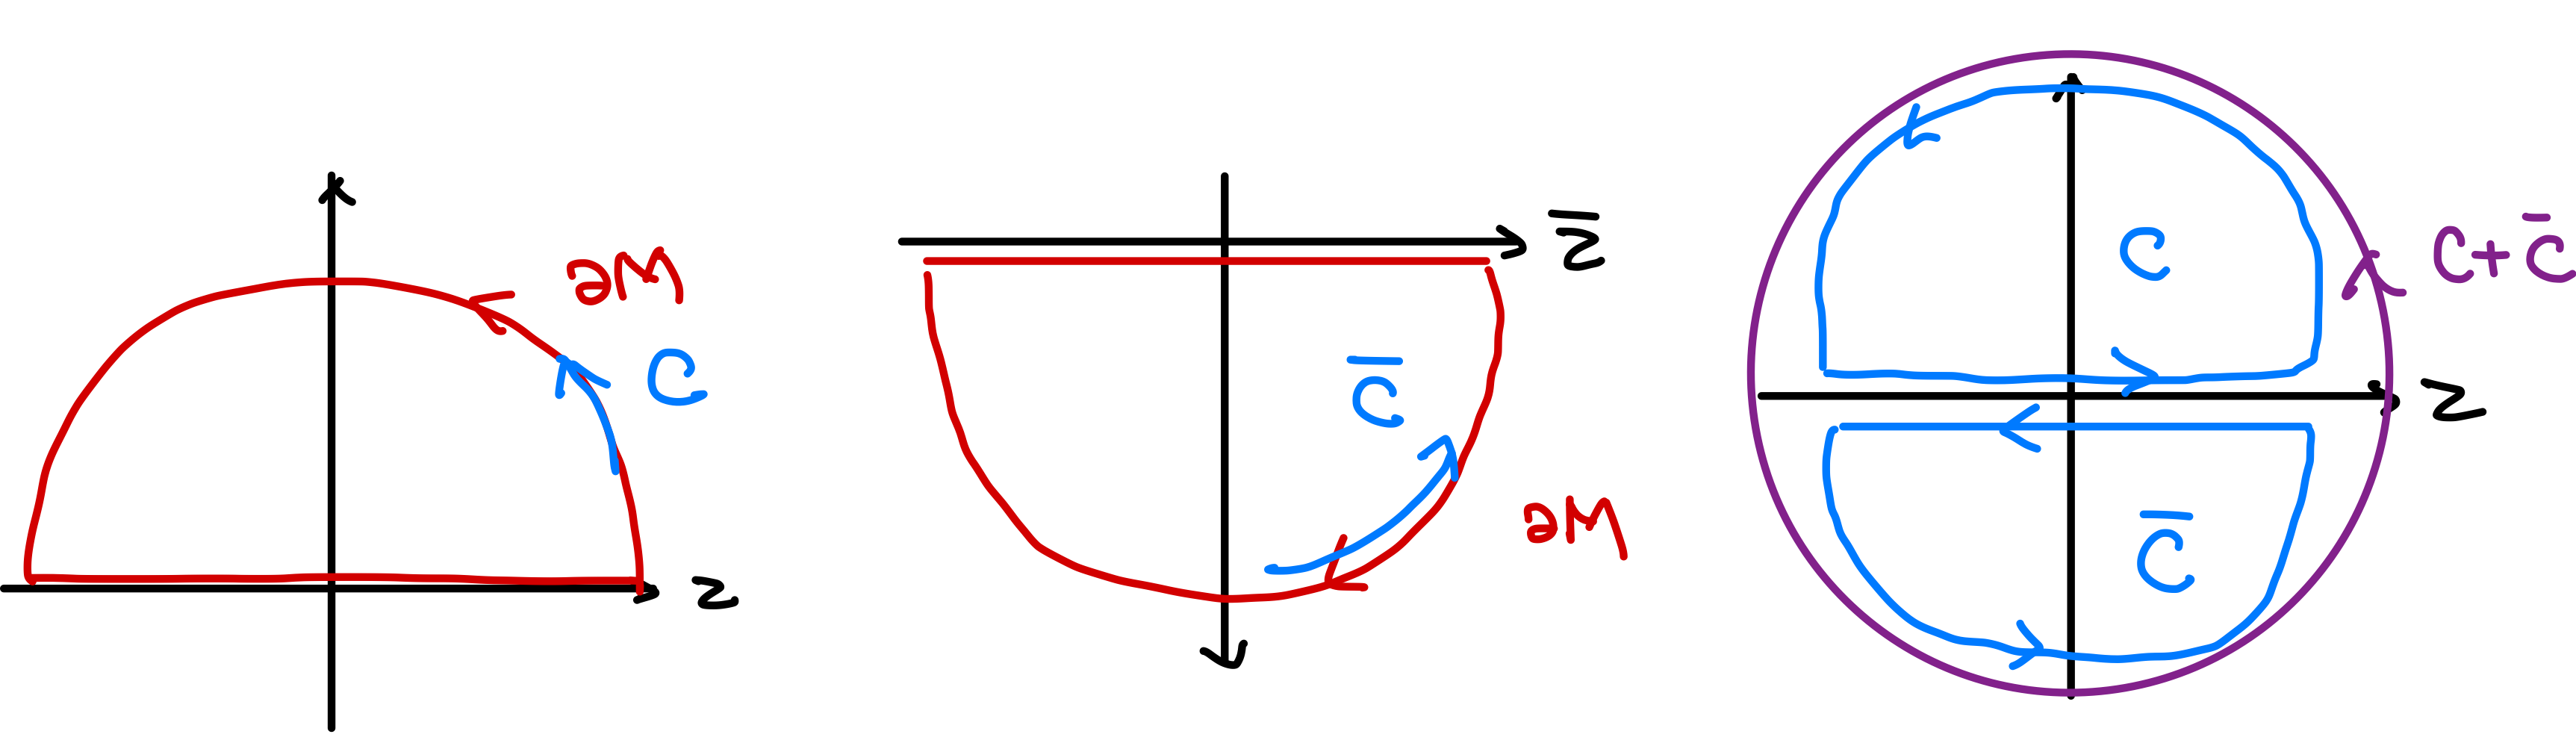
\includegraphics[width=0.75\textwidth]{assets/newontour.png}
  \caption{Choice of contour for conformal Ward identity on UHP after
  analytic continuation.}
  \label{fig:newontour}
\end{figure}
For Primary Field we can also do a similar trick to the LHS of the
conformal Ward identity. We have:
\begin{align}
  LHS=&-\frac{1}{2\pi
  i}\oint_{C^+}dw\mathrm{~}\epsilon(w)\sum_{i=1}^n\left[\frac{1}{w-z_i}\partial_{z_i}+\frac{h_i}{(w-z_i)^2}\right]\langle
  X\rangle_H\\
  &-\frac{1}{2\pi
  i}\oint_{\bar{C}^+}d\bar{w}\mathrm{~}\bar{\epsilon}(\bar{w})\sum_{i=1}^n\left[\frac{1}{\bar{w}-\bar{z}_i}\partial_{\bar{z}_i}+\frac{\bar{h}_i}{(\bar{w}-\bar{z}_i)^2}\right]\langle
  X\rangle_H\\
  =&-\frac{1}{2\pi
  i}\oint_{C^++\bar{C}^+}dw\mathrm{~}\epsilon^H(w)\sum_{i=1}^n\left[\frac{1}{w-z_i}\partial_{z_i}+\frac{h_i}{(w-z_i)^2}+\frac{1}{w-\bar{z}_i}\partial_{\bar{z}_i}+\frac{\bar{h}_i}{(w-\bar{z}_i)^2}\right]\langle
  X\rangle_H
\end{align}
Thus, we now have the conformal Ward identity on UHP:
\thm{
  \textbf{Conformal Ward Identity of Primaries on UHP}

  On UHP, for a set of primary fields $ X = \prod_{i=1}^n
  \phi_i(z_i,\bar{z}_i) $ , we have the conformal Ward identity:
  \begin{align}
    \langle T^H(z) X \rangle_{H} = \sum_{i=1}^n \left[ \frac{1}{z -
      z_i} \partial_{z_i} + \frac{h_i}{(z - z_i)^2} + \frac{1}{z -
      \bar{z}_i} \partial_{\bar{z}_i} + \frac{\bar{h}_i}{(z -
    \bar{z}_i)^2} \right] \langle X \rangle_{H}
  \end{align}
  where $ z \in \mathbb{C} $ and $ T(z) $ is the analytical continued
  E-M tensor.
}
\rmk{
  Attention that on the above equation $ z_i  \in \text{UHP} $
  however, $ z \in \mathbb{C} $. they have different domains.
}
Additionally, we can also assume the conformal Ward identity holds
for more general fields beyond primaries on UHP as well:
\axm{\label{axm:conformal ward identity UHP}
  \textbf{Conformal Ward Identity on UHP}

  On UHP, for a general set of fields $ X $, we have the conformal
  Ward identity:
  \begin{align}
    \delta_{\epsilon^H} \langle X \rangle_{H} = -
    \displaystyle\frac{1}{2 \pi i} \oint_{C^++\bar{C}^+}
    \epsilon^H(z) \langle T^H(z) X \rangle_{H}
  \end{align}
  where $ z \in \mathbb{C} $ and $ T^H(z) $ is the analytical
  continued E-M tensor.
}

\subsection{The Method of Images (Doubling Trick)}\label{sec:Method of Images}

The above discussion have give us a hint that the coorelation on the
UHP bahave as if we have twice the number of fields on the whole
complex plane. We observe the difference between the whole conformal
Ward identity on UHP and the holomorphic conformal ward identity on
the whole complex plane for primary fields:
\begin{align}
  \langle T(z) X_0 \rangle_{\mathbb{C}}& = \sum_{i=1}^n \left[
    \frac{1}{z - z_i} \partial_{z_i} + \frac{h_i}{(z - z_i)^2} +
    \frac{1}{z - \bar{z}_i} \partial_{\bar{z}_i} + \frac{\bar{h}_i}{(z
  - \bar{z}_i)^2}\right] \langle X_0 \rangle_{\mathbb{C}}\\
  \langle T^H(z) X \rangle_{H} &= \sum_{i=1}^n \left[ \frac{1}{z -
    z_i} \partial_{z_i} + \frac{h_i}{(z - z_i)^2} + \frac{1}{z -
    \bar{z}_i} \partial_{\bar{z}_i} + \frac{\bar{h}_i}{(z -
  \bar{z}_i)^2}\right] \langle X \rangle_{H}
\end{align}
Where we have:
\begin{align}
  X_0 &= \prod_{i=1}^n \phi_i(z_i) \prod_{i=1}^n
  \bar{\phi}_i(\bar{z}_i), \quad z_i , \bar{z}_i \in \mathbb{C} ,
  z_i^* = \bar{z}_i \\
  X &= \prod_{i=1}^n \phi_i(z_i,\bar{z}_i) , \quad z_i \in \text{UHP}
  , \bar{z}_i = z_i^* \in \text{LHP}
\end{align}
Where $ \phi_i(z_i) $ are chiral fields with conformal dimension $
(h_i,0) $ and $ \bar{\phi}_i(\bar{z}_i) $ are anti-chiral fields with
conformal dimension $ (\bar{h}_i, 0) $. We assume that they are all
holomorphic fields.
\begin{itemize}
  \item We can see that the \textbf{correlation function of the
    primaries on the UHP} satisfies the same differential equations
    as the \textbf{correlation function of twice of the number of
    chiral holomorphic fields on the whole complex plane}.
\end{itemize}
\rmk{
  By the word "chiral holomorphic fields" we mean the fields with
  conformal dimension $ (h,0) $ only and depends only on $ z $.

  In fact, chiral holomorphic fields can be physical, for example the
  majorana fermion field $ \phi(z) $ can be a $ (1/2,0) $ chiral
  holomorphic field.
}

By the procudure of getting the 2 point and 3 point function, we know
that the correlation function are determined by solving the conformal
ward identities. Thus, we can conclude that:
\thm{
  \textbf{Method of Images (Doubling Trick)}

  The \textbf{correlation function} of a set of primary fields $ X =
  \prod_{i=1}^n \phi_i(z_i,\bar{z}_i) $ on UHP
  \[
    =
  \]
  $ \sum $ of the \textbf{chiral conformal blocks} of twice the
  number of chiral holomorphic fields $ X_0 = \prod_{i=1}^n
  \phi_i(z_i) \prod_{i=1}^n \bar{\phi}_i(\bar{z}_i) $ on the whole
  complex plane.
}
Proof: this is a straightforward result of the definition of
conformal blocks and the above discussion.

An example is that the 1-point correlation function on UHP can be
computed via the 2-point chiral conformal blocks on the whole complex plane:
\begin{align}
  \langle \phi(z,\bar{z}) \rangle_{H} = \langle \phi(z)
  \bar{\phi}(\bar{z}) \rangle_{\mathbb{C}} \sim \frac{1}{(z -
  \bar{z})^{2h}} \text{ for } h = \bar{h}
\end{align}
There will be some constant prefactor to be determined by the theory
and the boundary condition on the boundary.

\newpage
\section{BCFT in Canonical Formalism}

\subsection{Radial Quantization with Boundary}

In the context of BCFT, we can also perform the Radial Quantization.
However, the equal-time slices are now semi-circles instead of full
circles due to the presence of the boundary. Other tahn this the
strategy of canonical quantization is similar to the ordinary CFT:
\begin{itemize}
  \item Radial Ordering
  \item OPE and Commutators relation
    ...
\end{itemize}

\subsubsection{Symmetry Algebra with Boundary}

Then we start to study the symmetry algebra with boundary. We notice
that from the general conformal Ward identity on UHP
\cref{axm:conformal ward identity UHP}, and the relation between the
commutators and the OPE, we then have:
\begin{align}\label{eq:generatorwithboundary}
  \delta_{\epsilon^H} \phi(w,\bar{w}) = - [Q_{\epsilon^H},
  \phi(w,\bar{w})] =- \oint_{C} \frac{dz}{2\pi i} \epsilon^H(z)
  T^H(z) \phi(w,\bar{w})
\end{align}
The integral contour is around the origin with both $ w $ and $
\bar{w} $ inside of it. Then we can expand $ \epsilon^H(z) $ and just
as the ordinary CFT case we can give out the generators as:
\begin{align}
  L_n^H = \frac{1}{2\pi i} \oint_{C} dz \ z^{n+1} T^H(z) =
  \oint_{C^+} \frac{dz}{2\pi i} z^{n+1} T(z) + \oint_{\bar{C}^+}
  \frac{d\bar{z}}{2\pi i} \bar{z}^{n+1} \bar{T}(\bar{z})
\end{align}
Just as the ordinary CFT case, we can compute the commutators between
these generators via the OPE of $ T^H(z) $ with itself. We have:
\thm{
  \textbf{Symmetry Algebra with Boundary}

  The generators $ L_n^H $ defined above satisfy the Virasoro Algebra:
  \begin{align}
    [L_n^H, L_m^H] = (n - m) L_{n+m}^H + \frac{c}{12} n (n^2 - 1) \delta_{n+m,0}
  \end{align}
}
We can see that now the symmetry algebra of the BCFT is just a single
copy of the Virasoro Algebra instead of two copies as in ordinary CFT.

\subsubsection{Hamiltonian on a semi-circle}
We then consider the Hamiltonian on a semi-circle. We consider the
integral on a semi-circle. We name the contour as $ S $ which is the
semi-circle part of $ C^+ $ with the same orientation as $ C^+ $ and
the contour $ \bar{S} $ which is the semi-circle part of $ \bar{C}^+
$ with the opposite orientation as $ \bar{C}^+ $.

The Hamiltonian of a theory should be given by the generator of the
"time" diraction. In CFT radial quantization, it is defined to be the
generator of the dilation transformation.
\rmk{
  It is important we define the Hamiltonian as the generator in time
  direction in the following style:
  \begin{align}
    - \partial_t \psi = \delta \psi = -[H, \psi]
  \end{align}
  Stick to this convention will avoid many confusions.
}
Considering the BCFT case \cref{eq:generatorwithboundary}, we have:
\thm{
  \textbf{Hamiltonian on Semi-circle}

  The Hamiltonian on a semi-circle is defined as:
  \begin{align}
    H^H =& \frac{1}{2\pi i} \oint_{S} dz\  z T(z) + \frac{1}{2\pi i}
    \oint_{\bar{S}} d\bar{z}\  \bar{z} \bar{T}(\bar{z})\\
    =& \frac{1}{2\pi i} \oint_{S + \bar{S} = C} dz \ z T^H(z)\\
    =& L_0^H
  \end{align}
  where $ L_0^H $ is the mode expansion of the analytical continued E-M tensor.
}
Proof: given by straightforward calculation, plug in the diation $
\epsilon^H(z) $we can get this generator from \cref{eq:generatorwithboundary}.

We will take this as a Hamiltonian of the BCFT.

\subsubsection{Hilbert Space Structure with Boundary}

Similarly, the Hilbert Space structure should take as the
representation of a single copy of the Virasoro Algebra. Thus, we have:
\thm{
  \textbf{Hilbert Space Structure with Boundary}

  The Hilbert Space of the BCFT is spanned by the highest weight
  representations of a single copy of the Virasoro Algebra:
  \begin{align}
    \mathcal{H}_\alpha = \bigoplus_{h} n^{h}_\alpha \mathcal{V}_h
  \end{align}
  where $ n_h $ are non-negative integers indicating the multiplicity
  of the representation $ \mathcal{V}_h $ in the Hilbert Space. Here
  we use $ \alpha $ to indicate the boundary condition of the BCFT.
}
Then we expect to construct this Hilbert Space via acting operators
on the vaccum state. However, we might face contraditions here, if we
nively act a bulk primary field $ \phi(z,\bar{z}) $ on the vacuum
state $ |0\rangle $, then it transforms as a representation of two
copies of the Virasoro Algebra instead of a single copy. Thus, the
state-operator correspondence seems to be less obvious here.

\subsection{Boundary Operators}

\subsubsection{Boundary Operators}

In section \cref{sec:Method of Images} we have seen that the one
point correlation function on UHP can be computed via the two-point
chiral conformal blocks on the whole complex plane. The correlation
function of single bulk field behave divergence as it approaches the
boundary. This phenomenon indicates that there may exist some new
fields living on the boundary to interact with the bulk fields.
\rmk{
  In QFT, we understand divergence by revealing hidden existence of new fields.
}
\defi{
  \textbf{Boundary Fields}

  The fields living on the boundary of a BCFT are called Boundary
  Fields. We denote them as $ \psi(x) $ where $ x \in \mathbb{R} $ is
  the coordinate on the boundary.
  Here we have some defining conditions for the boundary fields:
  \begin{itemize}
    \item They should be Chiral Fields with conformal dimension $ h $
      only and can be decomposed into primaries and descendants.
    \item $ h $ should be in the parent CFT's operator algebra content
    \item OPE of primary boundary fields with the E-M tensor behave as:
      \begin{align}
        T^H(z) \psi(x) = \frac{h}{(z - x)^2} \psi(x) + \frac{1}{z -
        x} \partial_x \psi(x) + \text{regular terms}
      \end{align}
      we can only consider the holomorphic part approaching from the UHP.
    \item OPE ensures that the commutation relation with the symmetry
      algebra as:
      \begin{align}
        [L_n^H, \psi(x)] = x^{n} (x \partial_x + (n+1) h) \psi(x)
      \end{align}
  \end{itemize}
}

%\question{
%   Why we must have boundary fields as this???
% }
%
% \YL{[I haven't fully understand this topic yet. I'm not sure why we
% must have boundary fields like this?]}

\subsubsection{Bulk-Boundary OPE}

The divergence behavior of bulk fields approaching the boundary
indicates that there should exist some relation between bulk fields
and boundary fields. This relation is given by the Bulk-Boundary OPE:
\thm{
  \textbf{Bulk-Boundary OPE}

  Bulk field should have the following behaviour as apporaching the boundary:
  \begin{align}
    \phi(z,\bar{z}) \sim \sum_{i} C_{(h,\bar{h}) i}^{\alpha}
    (2y)^{h_i - h - \bar{h}} \psi_i(x) \quad \text{as } y \to 0
  \end{align}
  where $ \alpha $ indicates the boundary condition, $ z = x + i y $,
  $ \psi_i(x) $ are boundary fields with conformal dimension $ h_i $
  and $ C_{\phi i}^{\alpha} $ are the bulk-boundary structure
  constants depending on the boundary condition.
}

This is really a general form of a standar OPE of two fields. It is
much an assumption that a derived result.

\subsection{Hilbert Space from Boundary Fields}

Now we can see that the construction of the Hilbert Space and the
manifestation of the state-operator correspondence in BCFT should be
done via the boundary fields instead of the bulk fields. We have:
\thm{
  \textbf{State Operator Correspondence in BCFT}

  The Hilbert Space of the BCFT can be constructed via acting
  boundary fields on the vacuum state:
  \begin{align}
    \ket{h} = \psi_h(0) \ket{0}
  \end{align}
}
This construction is valid for:
\begin{itemize}
  \item The state $ \ket{h} $ indeed is a primary state with
    conformal dimension $ h $. due to the commutation relation
    between the boundary fields and the symmetry algebra.
  \item The Bulk Operator can be expanded via the boundary operators
    as it approaches the boundary due to the Bulk-Boundary OPE.
\end{itemize}
Thus we believe that the Hilbert Space structure given above is valid.

% \question{
%   I'm not sure whether all operators acting on vaccum can be viewed
%   this way with these arguments?? Nor we know less about the
%   completness of boundary operators??
% }
%
% \question{what is the state of acting a bulk operator on the
%   vacuum??? it seems not able to be classified by the representations
% of Virasoro algebra alone???}
% A guess may be given by the description of Boundary State by
% Bulk-Boundary OPE ... But no book give this result??????

\subsection{CFT on a Strip}

\subsubsection{Transform to a Strip}

Now consider a more general case of boundary condition. We never said
that the boundary can only contain 1 single boundary condition. We
then have to think about what happens if there are more than 1. To
motivate the picture, we conformally map the CFT on the UHP minus the
origin to a strip. We define the following mapping.
\defi{
  \textbf{Mapping to a Strip}

  We define the conformal transformation of $ \mathbb{H}/\{0\} \to
  \text{Strip} $ as the following:
  \begin{align}
    t-i \sigma = w = \displaystyle\frac{L}{\pi} ln (z),\quad  x+iy =
    z \in \mathbb{H}
  \end{align}
}
The following diagram illustrate the process:

\begin{figure}[H]
  \centering
  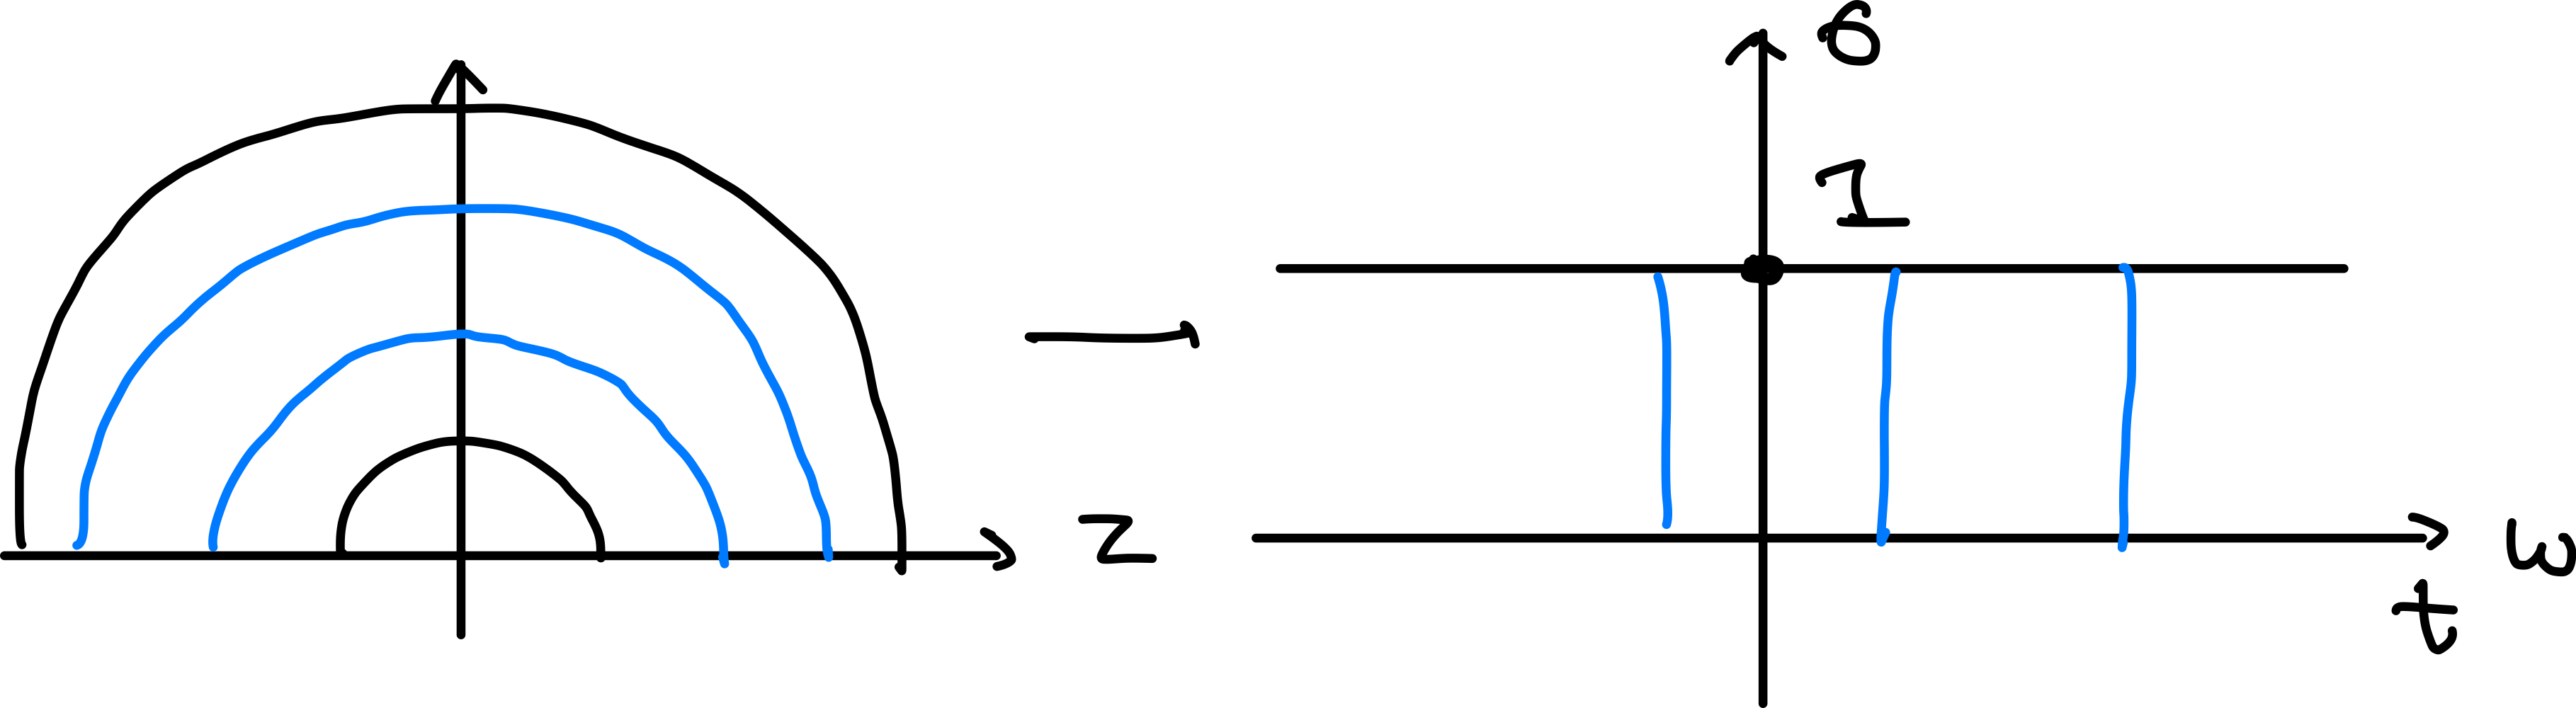
\includegraphics[width=0.75\textwidth]{assets/striptrans.png}
  \caption{Transformation to a Strip (there's a mistake in the
  diagram, it should be $ -\pi \to 0 $ on the $ \sigma $ axis )}
  \label{fig:striptrans}
\end{figure}
We then transform the fields on the UHP to the Strip:
\begin{align}
  &\phi^{S}(w,\bar{w})
  = \left( \frac{dw}{dz} \right)^{-h}
  \left( \frac{d\bar{w}}{d\bar{z}} \right)^{-\bar{h}}
  \phi^{H}(z,\bar{z})
  = (\alpha z)^{h} (\alpha \bar{z})^{\bar h}\, \phi^{H}(z,\bar{z}),
  \qquad \alpha = \frac{\pi}{L},
  \\
  &T^{S}(w)
  = \left( \frac{dw}{dz} \right)^{-2}
  \left( T(z) - \frac{c}{12} \{ w , z \} \right)
  = \alpha^{2} \left( z^{2} T(z) - \frac{c}{24} \right),
  \\
  &\bar T^{S}(\bar w)
  = \left( \frac{d\bar w}{d\bar z} \right)^{-2}
  \left( \bar T(\bar z) - \frac{c}{12} \{ \bar w , \bar z \} \right)
  = \alpha^{2} \left( \bar z^{2} \bar T(\bar z) - \frac{c}{24} \right).
\end{align}
Note that here we use the concrete $ T(z) $ and $ \bar{T}(\bar{z}) $
instead of the analytical continued one for clarity.

\subsubsection{Hamiltonian on a Strip}

\rmk{
  \textbf{What is the Hamiltonian?}

  There are many seemingly equivalent definitions of the Hamiltonian in a QFT:
  \begin{itemize}
    \item Legendre Transformation of the Lagrangian
    \item Generator of the time translation
    \item Integral of the energy density $ T_{tt} $
  \end{itemize}
  The first one and the third one in trivially equivalent with the
  definition. However, naively, the legrendre transformation may not
  lead to the generator of time translation, with a lack of coefficient.

  However, in QM the importance of Hamiltonian is from the definition
  as the generator of time translation. Thus, we should always define
  the Hamiltonian as the generator of time translation as a
  fundamental definition and fix the convention from this!!
}

Then, we can compute the Hamiltonian on the strip, we have:
\thm{
  \textbf{Hamiltonian on a Strip}

  The Hamiltonian on a strip with width $ \pi $ is given by:
  \begin{align}
    H_{\alpha \beta}^S = \displaystyle\frac{\pi}{L} \left( L_0^H -
    \frac{c}{24} \right)
  \end{align}
  where $ L_0^H $ is the mode expansion of the analytical continued
  E-M tensor and $ \alpha , \beta $ indicate the boundary conditions
  on the two boundaries of the strip.
}

Proof: The Hamiltonian on the strip is given by the generator of the
translation along $ t $ direction. We have:
\begin{align}
  H_{\alpha \beta}^S = \int_{0}^{-L} d\sigma \left( T_{tt}(\sigma,t)
  \right) , \quad T_{tt} = T_{zz}+ T_{\bar{z}\bar{z}} =
  \displaystyle\frac{1}{-2 \pi}(T(w) + \bar{T}(\bar{w}))
\end{align}
\YL{[I come up with this argument myself, please have someone to
check this with me!!!]}
Thus we have:
\begin{align}
  H_{\alpha\beta}^S& =  \int_{0}^{-L} \displaystyle\frac{1}{2 \pi i}
  d\omega T^S(w) +  \int_0^{-L} \displaystyle\frac{1}{2 \pi i}  d
  \bar{\omega}\bar{T}^S(\bar{w}) \\
  &= \displaystyle\frac{1}{2 \pi i} \displaystyle\frac{\pi}{L}
  \int_{C^+} dz z T(z) +  \displaystyle\frac{1}{2 \pi i}
  \displaystyle\frac{\pi}{L}\int_{\bar{C}^+} d\bar{z} \bar{z}
  \bar{T}(\bar{z}) - \displaystyle\frac{1}{2 \pi}\frac{c}{12}
  \int_{0}^{L} \displaystyle\frac{\pi}{L}d\sigma \\
  &= \frac{\pi}{L} \left( L_0^H - \frac{c}{24} \right)
\end{align}
Notice that here we use $ d w = \displaystyle\frac{L}{\pi}
\displaystyle\frac{dz}{z} $

\rmk{
  \textbf{What is the Hamiltonian??}

  The hamiltonian is the generator of translation along the time
  direction. so we should define it as some operators that satisfy:
  \begin{align}
    [H, \phi(\sigma,t)] = \partial_t \phi(\sigma,t)
  \end{align}
  this is a convention in CFT.
}
\rmk{
  Sometimes we define the conformal transformation to a strip with
  width $ L = \pi$ . In this case the Hamiltonian will be:
  \begin{align}
    w =  ln (z) \quad \Rightarrow \quad H_{\alpha \beta}^S =  L_0^H -
    \frac{c}{24}
  \end{align}
  This is also a common convention. In the rest of this note we will
  use this convention for simplicity.
}

\rmk{
  We note that $ L_n $ operator only takes the interpretation of
  conformal generator \textbf{On the Plane Coordinate}. Though we can
  use these operator to represent the Hamiltonian on the strip.
}

\subsection{Boundary Condition Changing Operators}

\subsubsection{Boundary Condition Changing Operators}

Then it motivates to think that what happens if we have different
boundary conditions on the two boundaries of the strip. In this case,
if we map the theory back to the UHP, we will have 2 boundary
conditions on the real axis with a shift in the origin. To capture
the divergence on the origin, we need to introduce a new type of
operators called Boundary Changing Operators.

\defi{
  \textbf{Boundary Changing Operators}

  The operators that change the boundary condition from $ \alpha $ to
  $ \beta $ at a point on the boundary are called Boundary Changing
  Operators. We denote them as $ \psi_{\alpha \beta}(x) $ where $ x
  \in \mathbb{R} $ is the coordinate on the boundary.
}

\subsubsection{Hilbert Space with 2 Boundaries}

The Hilbert Space with 2 boundaries may primarily be different, we
use the following general notation to stand for it:
\defi{
  \textbf{Hilbert Space with 2 Boundaries}

  The Hilbert Space of the BCFT with boundary conditions $ \alpha $
  and $ \beta $ on the two boundaries is denoted as $
  \mathcal{H}_{\alpha \beta} $:
  \begin{align}
    \mathcal{H}_{\alpha \beta} = \bigoplus_{h} n^{h}_{\alpha \beta}
    \mathcal{V}_h
  \end{align}
  Here we use the notation $n_h^{\alpha \beta} $ to indicate the
  multiplicity of the representation $ \mathcal{V}_h $ in the Hilbert Space.
}

An explanation of why this might fall into Virasoro representation is
that we always assume that boundary condition is compatible with the
conformal symmetry.
However, having two boundary conditions makes the translation
symmetry along the boundary break down, thus we might not be that
sure about this.

% \YL{[Its not obvious that in this case we can also fall into Vir
% Algebra representations!!!]}
% \question{
%   It seems that we assume the Vir Algebra still may exit, but its not
%   obvious? when we can't translate along the boundary any more???
% }

\subsubsection{State-Operator Correspondence}

In this case, the conformal symmetry seems to break down more, we
don't have translation symmetry along the boundary any more.
\begin{itemize}
  \item In this case, there won't be a well-defined state-operator
    correspondence any more because of the breaking of translation
    symmetry along the boundary.
\end{itemize}


\subsubsection{How to think about BCCO}

Above discussion are "motivations" of defining such BCCO on the boundary. However, to define such operator, we should not think in a traditional QFT way but in a bootstrapping way. Give out assumptions and try to make everything consistent.

\newpage

\section{Boundary Conditions of BCFT}\label{sec:Bootstrapping BCFT} % (fold)

In above sections we learn that there are additional objects in BCFT
compared to the parent CFT, such as boundary conditions, boundary
fields, boundary changing operators. However, these objects can not
arbitrarily exist, they should satisfy some consistency conditions to
make the theory well-defined.

This section we will discuss what kinds of consistent boundary
conditions can exist for a given parent CFT. To charaterize the
boundary condition, we have a very elegant way of describing it,
which is asigning a special state to a boundary condition. This
special state is called the Boundary State.

\subsection{Partition Function of BCFT on a Strip}

\subsubsection{Partition Function on a Strip}

To construct a state that encode the boundary condition, we have to
consider a thermal partition function of the CFT. It is much more
convenient to define it with the cooridnate transformation to a
strip. Thus, we define the following partition function:
\defi{
  \textbf{Partition function of CFT on a Strip}

  Consider a CFT on a UHP with conformal generators $ \{L_n^H\} $.
  The thermal partition function on a strip with boundary conditions
  $ \alpha $ and $ \beta $ on the two boundaries is defined as:
  \begin{align}
    Z_{\alpha \beta} (\tau) = \mathrm{Tr}_{\mathcal{H}_{\alpha
    \beta}} e^{- 2 \pi (L_0^H - c/24) Im \tau} =
    \mathrm{Tr}_{\mathcal{H}_{\alpha \beta}} q^{L_0^H - c/24}
  \end{align}
  where $ \tau $ is the modular parameter of the strip and $ q = e^{2
  \pi i \tau} $.Here we have $ \tau $ to be pure imaginary.
  The geometry of the compactified strip defined above is one with
  circumference $ 2 \pi Im(\tau) $ and length $ \pi $.
}

\defi{
  \textbf{Partition Function of CFT on a Strip (General Definition)}

  In General, we can define a thermal partition function on a strip
  with the following statement. Consider a theory with Hamiltonian $
  H_{\alpha \beta}^S $ on a strip with boundary conditions $ \alpha $
  and $ \beta $ on the two boundaries, which means that:
  \begin{align}
    [H^S_{\alpha \beta}, \psi(x)] = \partial_t \psi(x)
  \end{align}
  We define the thermal partition function on the strip as:
  \begin{align}
    Z_{\alpha \beta} (\tau) = \mathrm{Tr}_{\mathcal{H}_{\alpha
    \beta}} e^{- \tau H_{\alpha \beta}^S}
  \end{align}
  Where, $ \tau $ characterizes the circumference of the
  compactified direction.
}

This thermal partition function has a geometric interpretation. It
can be viewed as a partition function on a cylinder where the
compartified direction is the Euclidean time direction and the
spatial direction is the strip direction. The two boundaries of the
strip are then the two boundaries of the cylinder with boundary
conditions $ \alpha $ and $ \beta $ respectively.

\subsubsection{Characters of Virasoro Algebra}

Then we can expand the partition function via the characters of the
representations of the Virasoro Algebra:
\defi{
  \textbf{Character of Virasoro Algebra}

  The character of a representation $ \mathcal{V}_h $ of the Virasoro
  Algebra is defined as:
  \begin{align}
    \chi_h(q) =& \mathrm{Tr}_{\mathcal{V}_h} q^{L_0 - c/24}\\
    =& q^{h - c/24} \sum_{N=0}^{\infty} p(N) q^{N}
  \end{align}
  where $ p(N) $ is the number of partitions of integer $ N $.
}

There is a Important property of the characters under modular transformation:
\thm{
  \textbf{Modular Transformation of Characters}

  Under the modular transformation $ \tau \to -1/\tau $, the
  characters transform as:
  \begin{align}
    \chi_h (e^{-2\pi i / \tau}) = \sum_{h'} S_{h}^{h'} \chi_{h'}
    (e^{2\pi i \tau})
  \end{align}
  where $ S_{h}^{h'} $ is the modular S-matrix of the parent CFT.
  Note that $ \chi_h $ is the same function.
}
It just shows that the characters form a representation of the
modular group, it behaves as a Covariant object under modular transformation.

We then can see that the thermal partition function can be expanded
via the characters:
\begin{align}
  Z_{\alpha \beta} (q) = \sum_{h} n_{\alpha \beta}^{h} \chi_h (q)
\end{align}
Where $ n_{\alpha \beta}^{h} $ are non-negative integers indicating
the multiplicity of the representation $ \mathcal{V}_h $ in the
Hilbert Space $ \mathcal{H}_{\alpha \beta} $.

\subsection{CFT on a (choped) Cylinder}

\subsubsection{Transformation to a Cylinder}

Apart from the above picture of thermal BCFT on a strip, now I want
to define a \textbf{Choped Parent CFT on a Annulus}. Consider the
\textbf{Parent CFT} which generator this BCFT. We can transform it to
a cylinder and chop it to match the geometry of the compactified strip.
We then have to define a parent CFT on a cylinder:

\defi{
  \textbf{Mapping Parent CFT to a Cylinder}

  The mapping from the complex plane to a cylinder is defined as:
  \begin{align}
    t - i\sigma = \xi = \displaystyle\frac{L}{2 \pi} \ln z, \quad z =
    x + iy \in \mathbb{C}
  \end{align}
}
\begin{figure}[H]
  \centering
  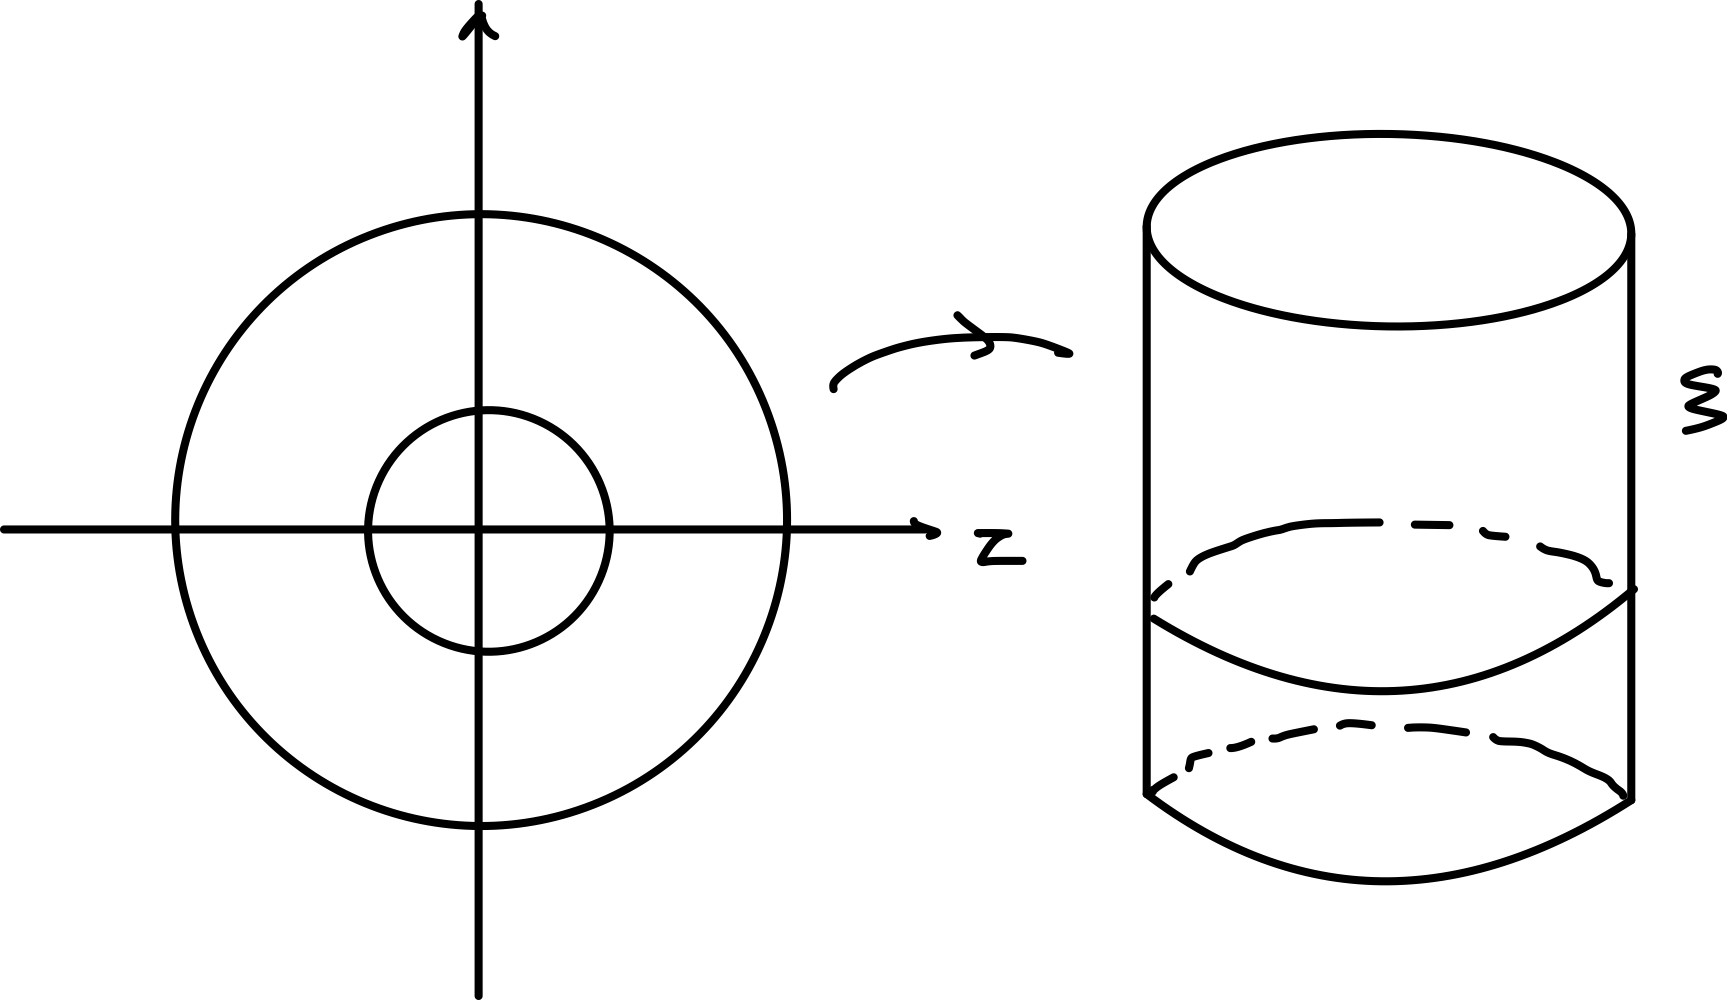
\includegraphics[width=0.4\textwidth]{assets/cftcyn.png}
  \caption{Mapping Parent CFT to a Cylinder}
  \label{fig:cftcyn}
\end{figure}
Under this mapping the E-M tensor transforms as:
\begin{align}
  \phi^C(\xi,\bar{\xi}) &= \left( \frac{d\xi}{dz} \right)^{-h} \left(
  \frac{d\bar{\xi}}{d\bar{z}} \right)^{-\bar{h}} \phi^P(z,\bar{z}) =
  \left( \frac{2\pi}{L} \right)^{h + \bar{h}} z^{h} \bar{z}^{\bar{h}}
  \phi^P(z,\bar{z})\\
  T^C(\xi) &= \left( \frac{d\xi}{dz} \right)^2 \left[ T^P(z) -
  \frac{c}{12} \{ \xi, z \} \right] = \left( \frac{2\pi}{L} \right)^2
  \left[ z^2 T^P(z) - \frac{c}{24} \right]\\
  \bar{T}^C(\bar{\xi}) &= \left( \frac{d\bar{\xi}}{d\bar{z}}
  \right)^2 \left[ \bar{T}^P(\bar{z}) - \frac{c}{12} \{ \bar{\xi},
  \bar{z} \} \right] = \left( \frac{2\pi}{L} \right)^2 \left[
  \bar{z}^2 \bar{T}^P(\bar{z}) - \frac{c}{24} \right]
\end{align}

\rmk{
  Recal different E-M tensor used in this section:

  E-M tensor of Parent CFT on complex plane: $ T^P(z) $;

  E-M tensor of Parent CFT on cylinder: $ T^C(\xi) $;

  E-M tensor of BCFT on UHP: $ T^H(z) $;

  E-M tensor of BCFT on strip: $ T^S(w) $.
}

\subsubsection{Hamiltonian of Parent CFT on a
Cylinder}\label{sec:Hamiltonian of Parent CFT on a Cylinder}

Then we derive the Hamiltonian on the cylinder:
\thm{
  \textbf{Hamiltonian of Parent CFT on Cylinder}

  The Hamiltonian of the Parent CFT on a cylinder with circumference
  $ L $ is given by:
  \begin{align}
    H^C = \frac{2\pi}{L} \left( L_0^P + \bar{L}_0^P - \frac{c}{12} \right)
  \end{align}
  where $ L_0^P , \bar{L}_0^P $ are the mode expansions of the
  holomorphic and anti-holomorphic E-M tensors of the Parent CFT on a
  complex plane.
}
Proof: The Hamiltonian on the cylinder is given by the generator of
the translation along $ t $ direction. We have:
\begin{align}
  H^C = \int_{0}^{-L} d\sigma \left( T_{tt}(\sigma,t) \right)
\end{align}

Then substituting the relation between $ T_{tt} $ and $ T^C(\xi),
\bar{T}^C(\bar{\xi}) $ we have:
\begin{align}
  T_{tt} = T_{\xi\xi} + T_{\bar{\xi}\bar{\xi}} =
  \displaystyle\frac{1}{-2 \pi}(T^C(\xi) + \bar{T}^C(\bar{\xi}))
\end{align}
Thus we have:
\begin{align}
  H^C& = \int_{0}^{-L} \displaystyle\frac{1}{2 \pi i}  d\xi T^C(\xi)
  +  \int_0^{-L} \displaystyle\frac{1}{2 \pi i}  d
  \bar{\xi}\bar{T}^C(\bar{\xi}) \\
  &= \displaystyle\frac{1}{2 \pi i} \displaystyle\frac{2 \pi}{L}
  \int_{C} dz z T^P(z) +  \displaystyle\frac{1}{2 \pi i}
  \displaystyle\frac{2 \pi}{L}\int_{\bar{C}} d\bar{z} \bar{z}
  \bar{T}^P(\bar{z}) - \displaystyle\frac{1}{2 \pi}\frac{c}{12}
  \int_{0}^{L} \displaystyle\frac{2 \pi}{L}d\sigma \\
  &= \frac{2\pi}{L} \left( L_0^P + \bar{L}_0^P - \frac{c}{12} \right)
\end{align}

\YL{[I come up with this argument myself, please have someone to
check this with me!!!]}
\rmk{
  \textbf{Discussion on the Normalization of the Hamiltonian on a Cylinder}

  The above proof contains many gaps, and in fact no standard
  textbook provides a fully rigorous derivation. The essential
  subtlety lies in the definition and normalization of the
  Hamiltonian on the cylinder. In practice, the Hamiltonian is
  defined with a specific normalization factor, which is finally
  fixed by demanding that the commutation relations generate the
  correct geometric transformations.

  We know that a correct generator must produce the correct
  transformation of fields through its commutators. Here, the
  Hamiltonian should generate translations along the Euclidean time
  direction $t$ on the cylinder. Thus we require
  \begin{align}
    [H_{\alpha\beta}^C , \phi^C(\xi,\bar{\xi})]
    = \partial_t \phi^C(\xi,\bar{\xi})
    = (\partial_\xi + \partial_{\bar{\xi}})\phi^C(\xi,\bar{\xi}).
  \end{align}
  This requirement fixes the normalization of the Hamiltonian. One
  may then verify that the definition of $H_{\alpha\beta}^C$ in terms
  of Virasoro generators indeed satisfies this condition. Therefore
  it is a valid Hamiltonian on the cylinder.

  However, checking this explicitly requires computing the commutator
  between $L_0$ and the cylinder field $\phi^C(\xi,\bar{\xi})$. This
  step is subtle because we must use
  \begin{align}
    [L_0, \phi^C(\xi,\bar{\xi})]
    &= [L_0^H, (\alpha z)^h (\alpha\bar{z})^{\bar{h}} \phi^P(z,\bar{z})] \\
    &= (\alpha)^{h+\bar{h}} z^h \bar{z}^{\bar{h}} ( z\partial_z + h )
    \phi^P(z,\bar{z}),
  \end{align}
  where $\alpha = \frac{2\pi}{L}$ and $z = e^{\alpha\xi}$.

  Now observe the identity
  \[
    z\partial_z\big( z^h \phi^P(z,\bar{z}) \big)
    = h z^h \phi^P(z,\bar{z})
    + z^h ( z\partial_z \phi^P(z,\bar{z}) ),
  \]
  which implies
  \begin{align}
    [L_0, \phi^C(\xi,\bar{\xi})]
    &= z\partial_z \big( (\alpha)^{h+\bar{h}}
    z^h\bar{z}^{\bar{h}}\phi^P(z,\bar{z}) \big)
    = \partial_\xi \phi^C(\xi,\bar{\xi}).
  \end{align}

  Thus the Hamiltonian must be proportional to the first-order operators:
  \[
    H = L_0 + \bar{L}_0 + \text{constant}
  \]
  and this fixes the overall normalization!!! Then we say that the
  overall constant comes from the transformation of the E-M tensor.
}

\rmk{
  \textbf{What is the Hamiltonian??}

  The hamiltonian is the generator of translation along the time
  direction. so we should define it as some operators that satisfy:
  \begin{align}
    [H, \phi(\sigma,t)] = \partial_t \phi(\sigma,t)
  \end{align}
  this is a convention in CFT.
}

\YL{[This important proof can be better organized]}

\subsubsection{Partition Function of a boundary Parent CFT on a Cylinder}

Then we can define the partition function of the Parent CFT on a
cylinder with states assigned to two boundaries:
\defi{
  \textbf{Partition function of Parent CFT on a Choped Cylinder}

  Consider a Parent CFT on a complex plane with conformal generators
  $ \{L_n^P\} , \{\bar{L}_n^P\} $. The partition function on a
  cylinder with states $ |\alpha \rangle , |\beta \rangle $ assigned
  to the two boundaries and the geometry of length $ a $ and
  circumfence $ L $ is defined as:
  \begin{align}
    Z_{\alpha \beta} (a,L) = \langle \alpha | e^{- a H^C} | \beta
    \rangle  \quad \text{ where } H^C = \frac{2\pi}{L} \left( L_0^P +
    \bar{L}_0^P - \frac{c}{12} \right)
  \end{align}
}
\begin{figure}[H]
  \centering
  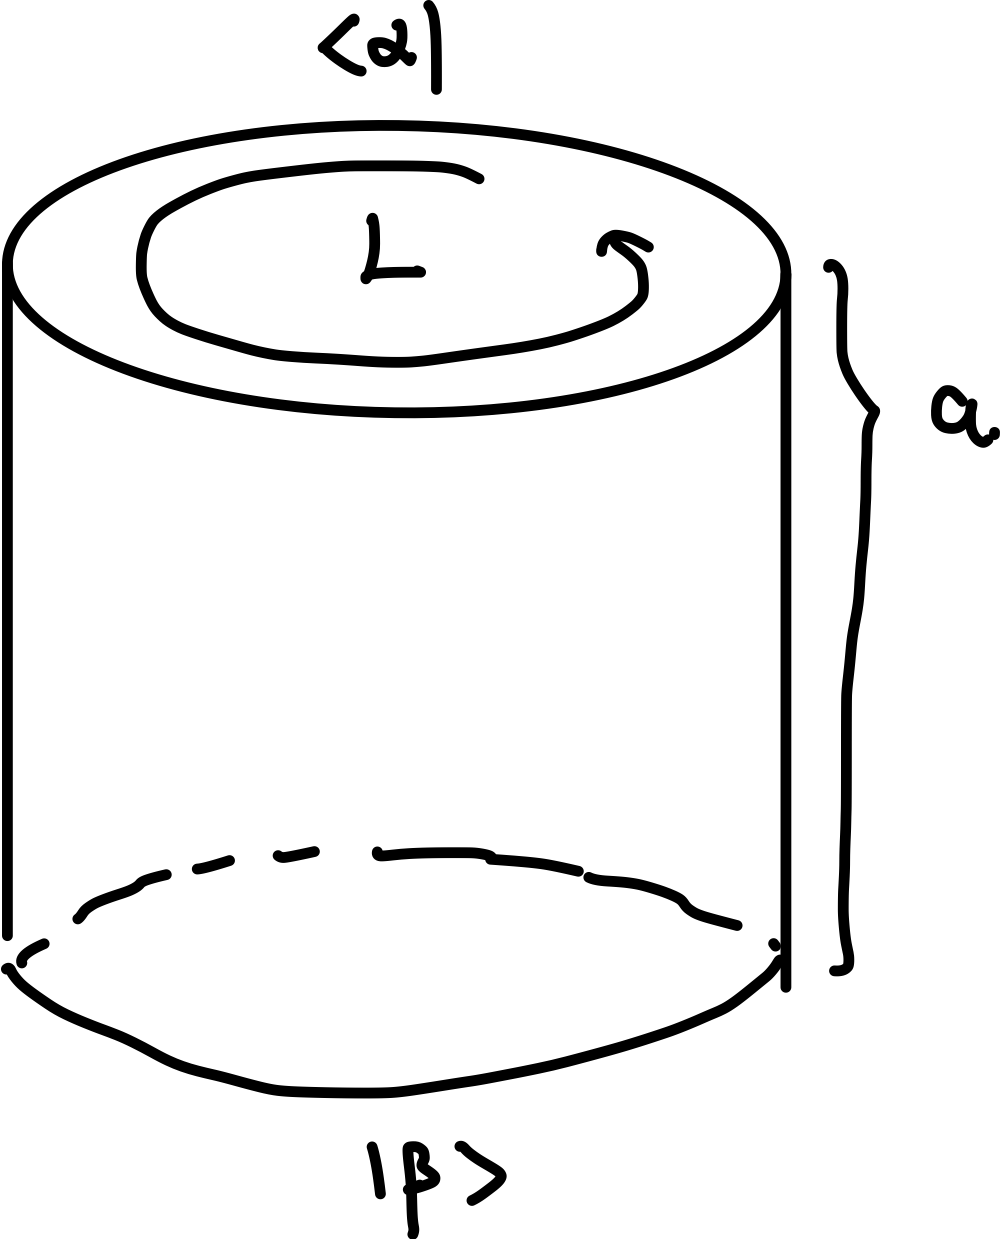
\includegraphics[width=0.2\textwidth]{assets/cylinder.png}
  \caption{Partition Function on a Cylinder}
  \label{fig:cylinder}
\end{figure}

However, this is a theory with boundaries, thus we need to impose the
gluing condition on the boundaries for the E-M tensor. There are two
different derivations of this condition:
\begin{itemize}
  \item Transform it into a UHP and transform the boundary to the
    real axis. Then impose the condition that there is no energy flow
    across the boundary, which gives $ T(z) = \bar{T}(\bar{z}) $ on
    the boundary. Transforming it back to the cylinder gives the
    gluing condition.

    \rmk{
      We shall note that we can't use the transformation $ w = \ln(z)
      $ here ,we have to let the boundary to be the real axis.
    }
  \item Consider that no energy flows across the boundary directly on
    the cylinder, which gives the same condition.
\end{itemize}
The condition is given by:
\thm{
  \textbf{Gluing Condition on a Cylinder}

  The gluing condition on a cylinder with boundaries assigned states
  $ |\alpha \rangle , |\beta \rangle $ is given by:
  \begin{align}
    (L_n^P - \bar{L}_{-n}^P) |\alpha \rangle = 0 , \quad (L_n^P -
    \bar{L}_{-n}^P) |\beta \rangle = 0
  \end{align}
}

Proof:
We want to proof the relation by transforming the gluing condition on
the UHP to a annulus on a complex plane. where the boundary meets the
boundary of the troped cylinder. just from a to c in the following diagram.
\begin{figure}[H]
  \centering
  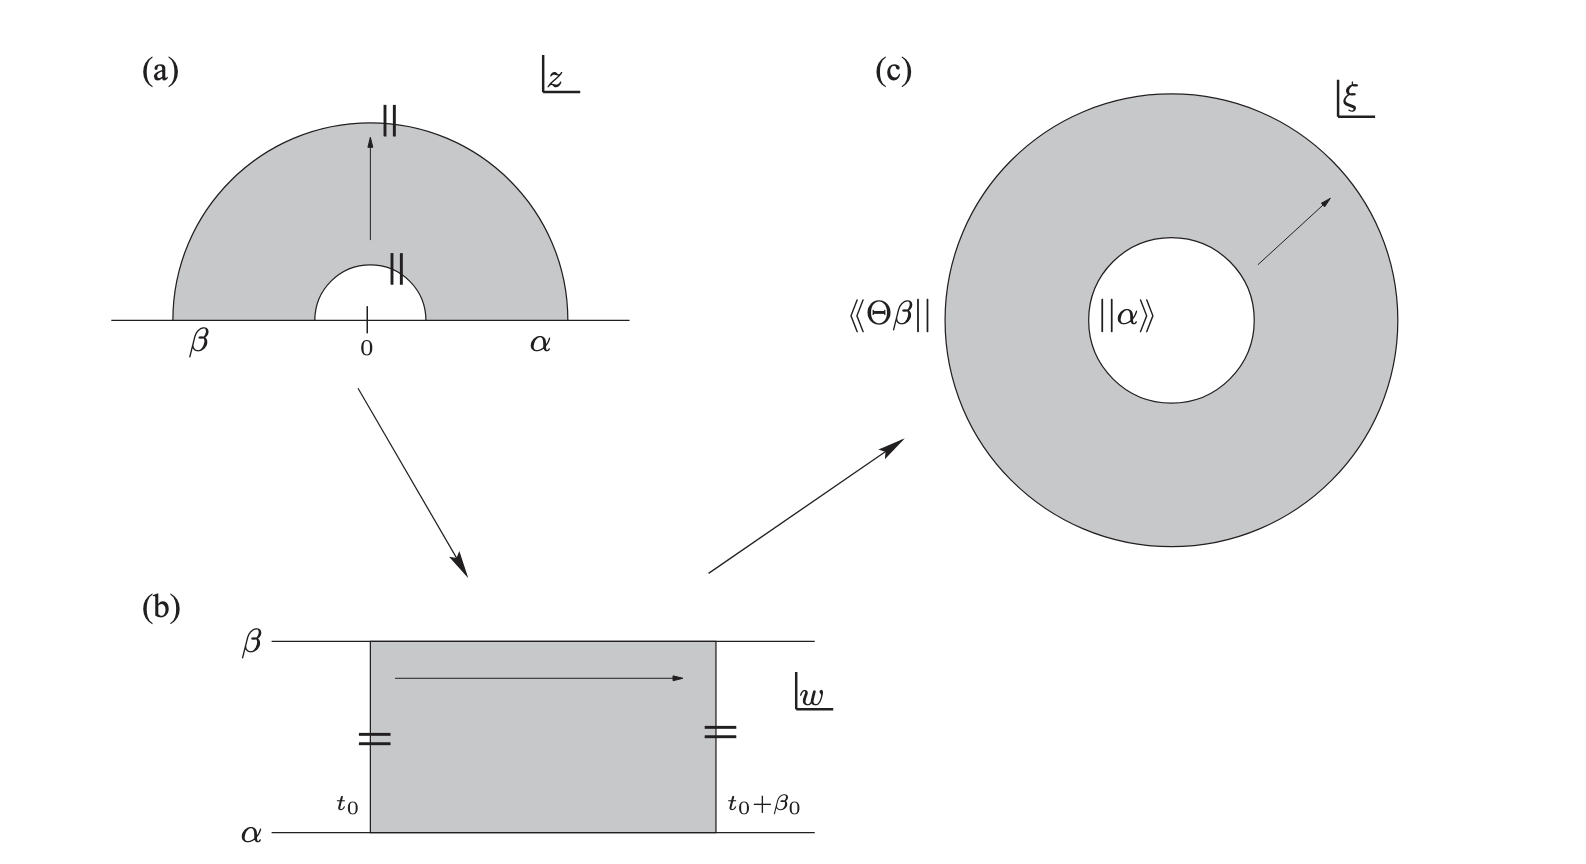
\includegraphics[width=0.75\textwidth]{assets/choptrans.png}
  \caption{Transformation from Cylinder to UHP}
  \label{fig:choptrans}
\end{figure}
\begin{itemize}
  \item\textbf{ Inner circle transfromation: } Inner circle $ |\xi| =
    1 $ maps to the boundary at $ z \in \mathbb{R}_+ $ of the cylinder;
\end{itemize}
We define the transformation for the inner circle from  as:
\begin{align}
  \xi=e^{\frac{2\pi i}{L}\ln z} \quad \bar{\xi}=e^{-\frac{2\pi
  i}{L}\ln \bar{z}}
\end{align}
This transformation has the following property on the boundary:
\begin{align}
  \bar{\xi}=\xi^{-1},\quad\left(\frac{d\bar{\xi}}{d\bar{z}}\right)\left(\frac{d\xi}{dz}\right)^{-1}=-\bar{\xi}^2,\quad\left\{\xi,z\right\}=\left\{\bar{\xi},\bar{z}\right\},
  z = \bar{z}
\end{align}
Thus the gluing condition on the UHP $ T^P(z) = \bar{T}^P(\bar{z}) $
transforms to:
\begin{align}
  \left[\left(\frac{d\xi}{dz}\right)^2T^{P}(\xi)-\left(\frac{d\bar{\xi}}{d\bar{z}}\right)^2\overline{T}^{P}(\bar{\xi})\right]
  = 0
\end{align}
Then we use the above properties and mode expand the gluing
condition, we can see that:
\begin{align}
  T^P(\xi, \bar{\xi}) - \bar{\xi}^4 \bar{T}^P(\bar{\xi}, \xi) =
  \sum_n \left( L_n^P - \bar{L}_{-n}^P \right) \xi^{-n-2} = 0
\end{align}
Finally, we can get that the gluing condition on the cylinder is given by:
\begin{align}
  (L_n^P - \bar{L}_{-n}^P) |\alpha \rangle = 0 , \quad (L_n^P -
  \bar{L}_{-n}^P) |\beta \rangle = 0
\end{align}

\begin{itemize}
  \item \textbf{Outerier circle transformation: }
\end{itemize}

\YL{[I still don't understand this proof very well... but it is claim
that this won't give out any new condition]}

\rmk{
  Personally, I'd rather think of the gluing condition as an assumption instead of a theorem of the theory, with this assumption connecting the parent CFT and BCFT, we may able to use the boundary state formalism.
}

\subsubsection{Ishibashi States}

States that satisfy the gluing condition are called Ishibashi States.
They can be constructed as follows:
\thm{
  \textbf{Ishibashi States}

  For each representation $ \mathcal{V}_h $ of the Virasoro Algebra
  of the Parent CFT, there exists a unique Ishibashi State $ |h
  \rangle \rangle $ satisfying the gluing condition:
  \begin{align}
    |h \rangle \rangle = \sum_{N} |h;N \rangle \otimes \overline{|h;N \rangle}
  \end{align}
}

\subsection{Boundary State Formalism}

\subsubsection{Definition of Boundary State}

With the preparation above, we then can fully define the Boundary
State. It is defined as follows:
\defi{
  \textbf{Boundary State}

  The boundar state is defined as a state on a boundary parent CFT on
  a cylinder $ \ket{\alpha}, \ket{\beta} $
  \begin{itemize}
    \item that has the same geometry as a compactified strip;
    \item and gives the same partition function as the thermal
      partition function of the BCFT on the strip with boundary
      condition $ \alpha, \beta $.
  \end{itemize}

  Here we assume the cylinde has length $ \pi $ and circumfence $ 2
  \pi Im(\tau) $ for simplicity. Thus, the boundary state $ |\alpha
  \rangle , |\beta \rangle $ assigned to the two boundaries is defined as:
  \begin{align}
    Z_{\alpha \beta} (\tau) = \mathrm{Tr}_{\mathcal{H}_{\alpha
    \beta}} q^{L_0^H - c/24} = \langle \alpha | e^{- \pi H^C} | \beta
    \rangle \quad \text{ where } H^C =
    \displaystyle\frac{1}{Im(\tau)} \left( L_0^P + \bar{L}_0^P -
    \displaystyle\frac{c}{12} \right)
  \end{align}
  The right hand side can also be written in a $ q = e^{2 \pi i \tau} $ style:
  \begin{align}
    Z_{\alpha \beta} =
    \langle\alpha|(\tilde{q}^{1/2})^{L_{0}^{(P)}+\overline{L}_{0}^{(P)}-c/12}|\beta\rangle,
  \end{align}
  where $ \tilde{q} = e^{-2\pi i / \tau}= e^{-2 \pi /Im(\tau)} $.
}

Boundary state is the state lives on the boundary of the Parent CFT
on a cylinder that encodes the boundary condition of the BCFT on a
strip. Thus, it should satisfy the gluing condition:
\begin{align}
  (L_n^P - \bar{L}_{-n}^P) |\alpha \rangle = 0 , \quad (L_n^P -
  \bar{L}_{-n}^P) |\beta \rangle = 0
\end{align}
So we have the conclusion that:
\thm{
  \textbf{Boundary State Expansion}

  The boundary state can be expanded via the Ishibashi states as:
  \begin{align}
    \ket{\alpha} = \sum_h |h \rangle \rangle  \langle\langle h |
    \alpha \rangle
  \end{align}
}

\subsubsection{Cardy Condition}

If the Parent CFT is a Diagnonal CFT, we can derive a very important
condition for the boundary states called the Cardy Condition and give
out an important solution to it. For a diagonal CFT, we have $ h =
\bar{h} $ for all primary fields.

Due to the property of the Diagonal CFT, we can rewrite the partition
function on a troped cylinder as:
\begin{align}
  Z_{\alpha \beta} =
  \langle\alpha|(\tilde{q}^{1/2})^{L_{0}^{(P)}+\overline{L}_{0}^{(P)}-c/12}|\beta\rangle
  = \sum_h \langle\alpha|h\rangle\rangle \langle\langle
  h|\beta\rangle \chi_h(\tilde{q})
\end{align}
Compare with the partition function on a strip and using the modular
transformation of characters, we have:
\thm{
  \textbf{Cardy Condition}

  The boundary states $ |\alpha \rangle , |\beta \rangle $ must
  satisfy the following condition:
  \begin{align}
    \sum_h \langle\alpha|h\rangle\rangle \langle\langle
    h|\beta\rangle S_{h}^{h'} = n_{\alpha \beta}^{h'}
  \end{align}
  or equivalently:
  \begin{align}
    \langle a|h^{\prime}\rangle\rangle\langle\langle
    h^{\prime}|b\rangle=\sum_hS_h^{h^{\prime}}n_{ab}^h.
  \end{align}
}
